%chapter 1
\chapter{Detection in Noble Fluids}
Noble fluids are very attractive materials for use when particle and radiation detection is required. They are commonplace in current detector technologies, with argon being the most prolific. It is hard to imagine in this modern era designing detectors and experiments without the use of noble fluids, and this chapter aims to motivate and describe their use.

%%Noble Gas Detectors
\section{The Noble Gases}
The five naturally occurring noble elements, excluding the radioactive radon (Rn), are helium (He), neon (Ne), argon (Ar), krypton (Kr) and xenon (Xe). Being chemically inert provides them with unique attributes that are key for particle detectors, specifically for detectors which collect charge and scintillation light. However some noble gas detectors can require extremely high purities, in excess of the order of 0.1 part per billion (ppb). Their properties relevant to detector design are shown in table~\ref{tab:nobelGasPara1}. 

\renewcommand{\arraystretch}{1.5}
\begin{table}
\begin{center}
  \begin{tabular}{l*{6}{c}r}
  \hline
  & \textbf{He} & \textbf{Ne} & \textbf{Ar} & \textbf{Kr} & \textbf{Xe} \\
  \hline
  Atomic number, Z & 2 & 10 & 18 & 36 & 54 \\
  Molar mass [g mol$^{-1}$] & 4.00 & 20.2 & 39.9 & 83.8 & 131 \\
  Density (273 K, 1 atm) [kg m$^{-3}$] & 0.179 & 0.888 & 1.76 & 3.70 & 5.90 \\
  Boiling point (1 atm) [K] & 4.40 & 27.1 & 87.3 & 112 & 169 \\
  Critical point: & & & & & \\
  \hspace{4mm} Temp [K] & 5.25 & 44.4 & 151 & 209 & 290\\
  \hspace{4mm} Pressure [MPa] & 0.226 & 2.69 & 4.90 & 5.43 & 5.76\\
  Triple point: & & & & & \\
  \hspace{4mm} Temp [K] & 2.18 & 24.6 & 83.8 & 115 & 161\\
  \hspace{4mm} Pressure [kPa] & 5.04 & 43.4 & 68.8 & 73.4 & 81.8 \\
  First excitation energy (293K, 1 atm) [eV] &19.8 & 16.7 & 11.6 & 10.5 & 8.4 \\
  Ionisation energy (293K, 1 atm) [eV] & 24.6 & 21.6 & 15.7 & 13.0 & 12.1\\
  Scintillation wavelength [nm] & 78 & 80 & 128 & 147 & 175\\
  Radiation length [g cm$^{-2}$] & 89.9 & 28.9 & 19.9 & 11.7 & 8.49 \\
  Abundance in atmosphere [ppm] & 5.20 &18.2 & 9340 & 1.10 & 0.09 \\
    \hline
  \end{tabular}
      \caption{ The properties of the 5 natural occurring non-radioactive nobel gases. Data taken from \cite{gasDetectors} and \cite{nobleGasDetectors}. Radiation lengths correspond to the most naturally abundant isotopes ($^{4}$He, $^{20}$Ne, $^{40}$Ar, $^{84}$Kr and$^{129}$Xe) and are calculated from an experimental fit from \cite{radiationLengthsBook}. Abundance in Earth's atmosphere given by \cite{nobleGasAbundance}.}
    \label{tab:nobelGasPara1}
\end{center}
    \end{table}
\renewcommand{\arraystretch}{1.0}

Natural abundance and ease of production drives the price of the gases. The lightest of the noble gases, He, Ne and Ar are the most abundant in the Earth's atmosphere. High abundance can result in low production costs and makes these three the most easily attainable of the noble gases. They are popular candidates for use in detectors, as vast quantities can be required for large detector volumes and for purification processes. Kr and Xe are much less abundant in the atmosphere and as a result are more expensive to produce. The global production of Xenon is $\sim$5 tonnes per year\cite{xenonProduction}, costing $\sim$\textsterling 1500 / liquid litre compared to Ar at $\sim$700,000 tonnes per year\cite{argonProduction}, costing $\sim$\textsterling 1.3 / liquid litre.

Other considerations must be taken into account for their use in detectors. The most important trait for use as a detector medium is the ability to absorb and efficiently measure energy transfer of incident particles or radiation. Heavier noble gases are preferable for this, with higher atomic numbers making it favourable for electromagnetic interactions. Noble fluids are usually implemented in either liquid or gaseous states, however since all the stable noble gases have boiling points below room temperature and pressure, cryogenics are usually required to maintain them in a liquid state. Gases can avoid the need for this, but require high pressures to achieve adequate detector efficiencies. The pressure is then a measure of controlling the density and hence their stopping power.
%As a consequence of this the control of the medium density is very desirable

It is also worth noting that some of these noble gases contain radioactive isotopes which can introduce unwanted backgrounds in detectors. Argon contains traces of $^{39}$Ar, which decaying via $\beta$-decay releases an energy of $\sim$0.5 MeV, which is a large background relevant for lower energy detectors. Krypton contains small amounts of $^{78}$Kr and $^{81}$Kr, which are also radioactive. Xenon has three naturally occurring isotopes that are radioactive, $^{124}$Xe, $^{134}$Xe and $^{136}$Xe, however these have such long lifetimes they can be considered stable. Traces of $^{85}$Kr ($\beta$-decay at 687 keV) are the most problematic of the radioactive contaminates for low energy xenon detectors.

The two main implementations of noble fluids as detector media are as Ionisation Detectors and Scintillation Detectors. These detection methods rely on the interaction of charged particles with atoms in the medium, causing ionisation or excitation. Neutral particles can be detected indirectly also by inferring their interaction from the propagation of charged particles in the volume. While ionisation and scintillator detectors are presented sequentially and independently, it can be beneficial to incorporate the two into a single detector technology, with some current and proposed detectors operating to utilise both methods of particle detection.
    
\section{Noble Gases as Ionisation Detectors}
Charged particles interact primarily with electrons in atoms while traversing matter. Moderately relativistic (0.05 $< \beta\gamma <$ 500) heavy charged particles such as $\mu$, $\alpha$, protons and nuclear ions, lose their energy according to the well described equation \ref{eq:betheFormula}, the Bethe-Bloch formula\cite{radiationLengthsBook}. 
\begin{equation}
	- \Big\langle\frac{dE}{dx}\Big\rangle = 4 \pi N_{A}r^{2}_{e}m_{e}c^{2}z^{2}\frac{Z}{A}\frac{1}{\beta^{2}}\Bigg[ \frac{1}{2} \textnormal{ln} \Big( \frac{2m_{e}c^{2}\beta^{2}\gamma^{2}T_{max}}{I} \Big) - \beta^{2} - \frac{\delta}{2} \Bigg]
	\label{eq:betheFormula}
\end{equation}
Here $\langle dE/dx\rangle$ is the mean rate of energy loss per unit length, where $N_{A}$ = 6.02214179(30) $\times$ 10$^{23}$ mol$^{-1}$ is the Avogadro constant, $r_{e}$ is the classical electron radius, $z$ is the charge of the incident particle in units of $e$ and with $\beta$ = $v/c$. The Lorentz factor is $\gamma$ = $1/\sqrt{1-\beta^{2}}$ and $I$ represents the mean excitation energy of the atom. The maximum kinetic energy that can be transferred from the incident particle, of mass $M$, to an electron, mass $m_{e}$, in a single collision is represented by $T_{max}$. This is determined by equation \ref{eq:betheMaxEnergy} \cite{radiationLengthsBook}. The $\delta$ factor is a correction factor for density effects. 
\begin{equation}
	T_{max} = \frac{2m_{e}c^{2}\beta^{2}\gamma^{2}}{1 + 2\gamma m_{e}/M + (m_{e}/M)^{2}}
	\label{eq:betheMaxEnergy}
\end{equation}
The energy loss for electrons in denser materials is mainly due to Bremsstrahlung and is not well described by the Bethe-Bloch equation but for cases when the mean free path is high then it can be considered minimum ionising. Application of this equation for heavy charged particles of interest such as muons, protons, pions, alpha particles and electrons can be seen over the energy range of 0.1 to 10$^{7}$ GeV in figure \ref{fig:betheEnergyLoss} for them traversing Argon.

\begin{figure}
\begin{center}
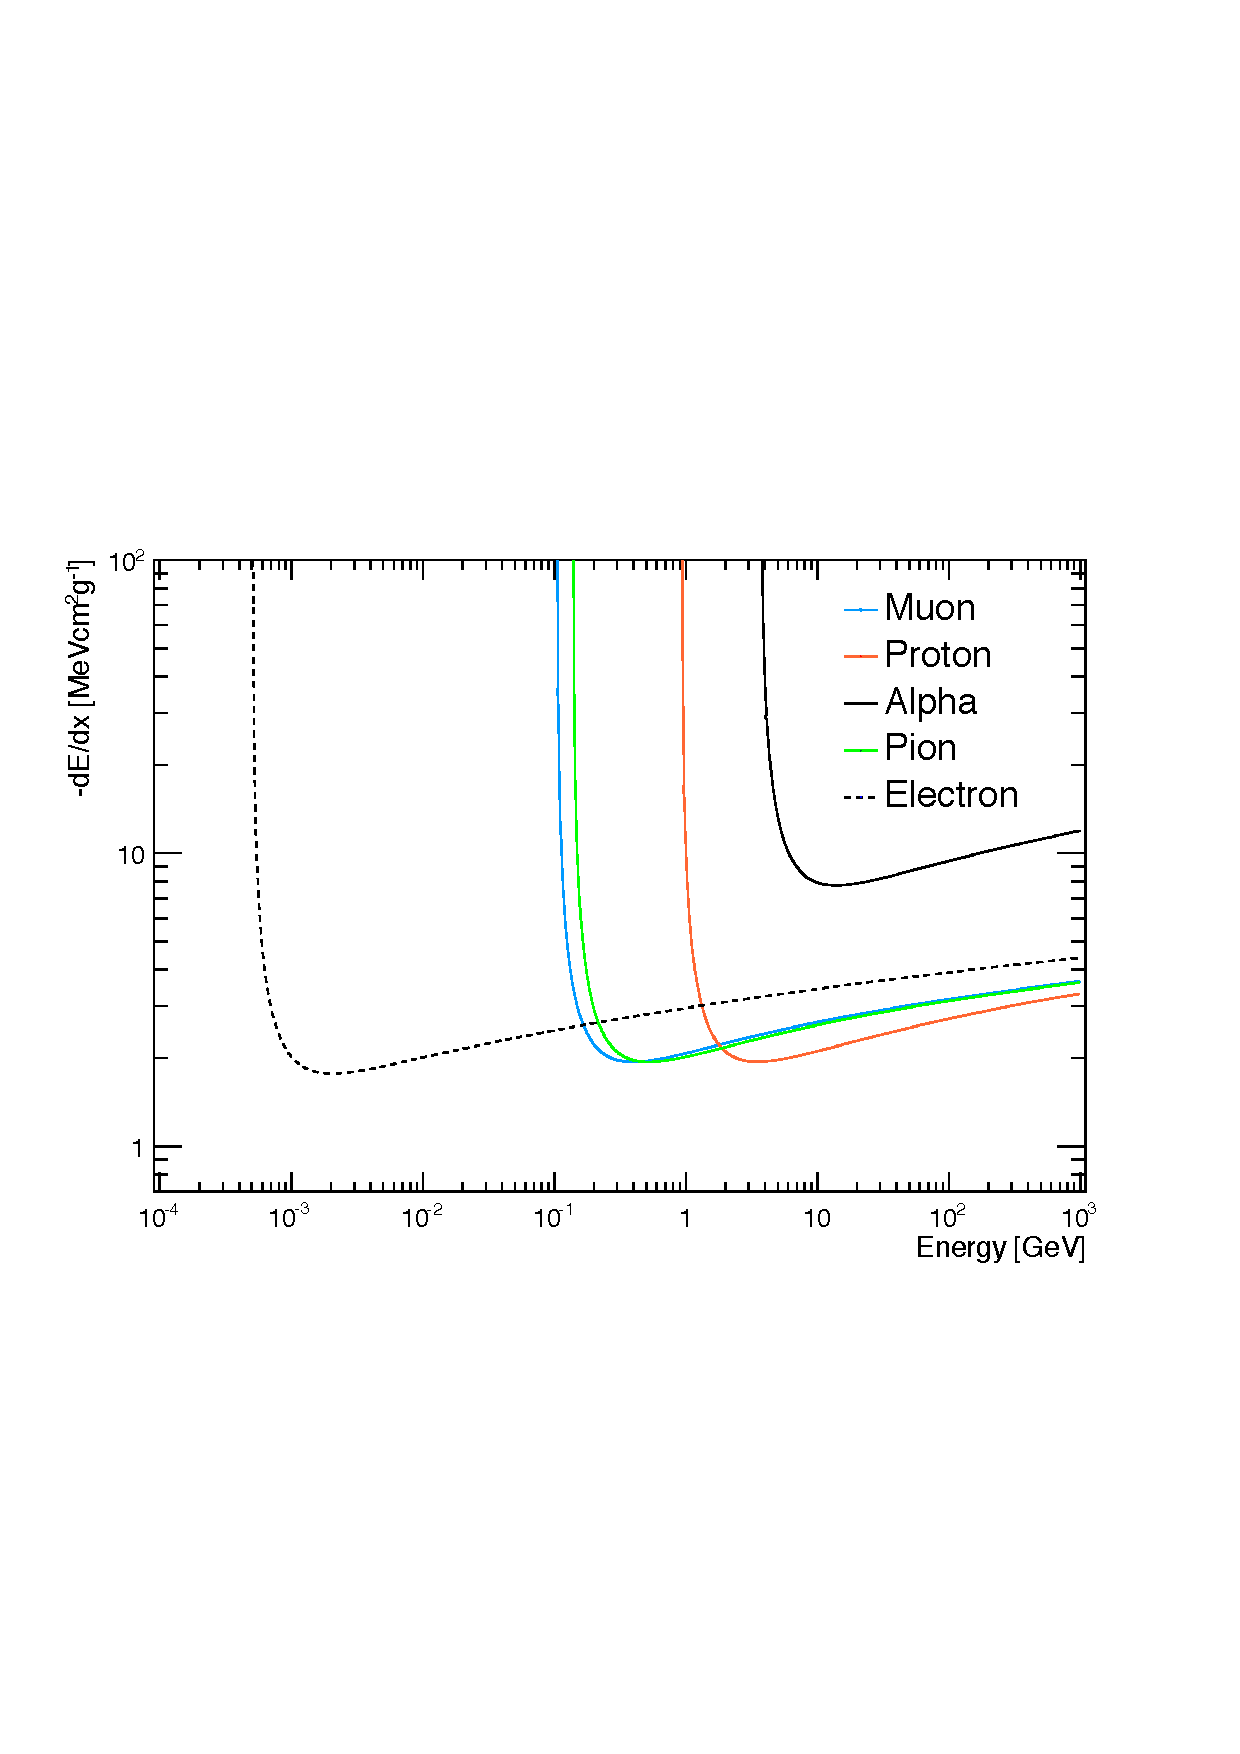
\includegraphics[width=100mm]{Chapter1/figures/energyLossInArgon.pdf}
\caption{The mean energy loss per unit length, $\langle dE/dx \rangle$, calculated from equation \ref{eq:betheFormula}, shown for muons, protons, charged pions, alpha particles and electrons in Argon at 293 K and 1 atm, which 11.6 eV was used as the excitation energy and $\delta$ = 0. }
\label{fig:betheEnergyLoss}
\end{center}
\end{figure}
The Bethe equation only describes the mean energy loss for moderately relativistic heavy charged particles. Particles with $\beta\gamma\lesssim$0.05 fall outside this description with nuclear effects more important and no analytical description of their energy loss is given. For highly relativistic charged particles of $\beta\gamma\gtrsim$500, radiative effects begin to have greater influence, with pair production and Bremsstrahlung the dominant processes. For muons and pions this limit is reached at around several hundred GeV. Such large energies are not considered in this thesis and focus is on the 0.2 to 10 GeV scale, in the minimum ionising regime. 

The heavy charged particle will interact with the electrons in the gas losing energy according to the equation \ref{eq:betheFormula} through the exchange of virtual photons. If the energy of such a photon is above the ionisation potential then this will cause ionisation. Further ionisation can occur from energetic electrons that escape the molecule, namely $\delta$-rays. The majority of $\delta$-rays will have small ranges compared to that of the incident charged particle, and ionisation remains close to the track.

On production of an ionisation pair, an electron and an ion, an electric field can be applied to the volume to introduce the drift of the electrons/ions, thus overcoming the Coulomb electron-ion attraction and ultimately reducing the recombination process. If purities and electric fields are high enough it then allows for the ability to drift over vast distances (several meters). Once charges have been drifted they can then be collected and read out, producing a two dimensional representation of the ionisation. 

The equation of motion of charged particles subject to electric, \textbf{E}, and magnetic, \textbf{B}, fields can be described by equation \ref{eq:eomDrift}, for a particle of velocity \textbf{v} of mass $m$ and charge $e$. A frictional force proportional to the velocity is represented by $K\textbf{v}$ to allow for interactions within the gas. The constant $K$ is given in terms of the mean time between collisions, $\tau$, with $K=m/\tau$, and drift velocities are calculated at times, t$\gg\tau$. It can be seen that if the magnetic field is non existent or perpendicular to the electric field then cross product effects are removed, resulting in a drift velocity that is independent of the magnetic field strength. This is a powerful technique as magnetic fields can also be required for momentum measurements in detectors.
\begin{equation}
	m\frac{d\textbf{v}}{dt} = e(\textbf{E} + \textbf{v} \times \textbf{B}) - K\textbf{v}
	\label{eq:eomDrift}
\end{equation}
The magnitude of the drift velocity can then be written as proportional to the electric field strength in the drift direction, $|\textbf{E}|\text{cos}{\phi}$, as in equation \ref{eq:driftVelocity}. The mobility is then defined as $\mu = e\tau/m$ \cite{driftDetectorsBook}.
\begin{equation}
	|\textbf{v}| = \frac{e}{m}\tau|\textbf{E}|\text{cos}{\phi}
	\label{eq:driftVelocity}
\end{equation}
With electrons far lighter than ions, they are favourable for drifting, this not only increases their mobility and acceleration due to the electric field but also reduces the energy loss due to collisions during drifts. The ability to drift electrons is a popular technique employed in many modern particle detectors. One of the dominant technologies in this field is the Time Projection Chamber (TPC). Argon and Xenon are the most favoured of the nobel gases for use in TPCs, due to their high densities and radio purities. Argon is far more common however, as it is far more abundant and therefore much cheaper for experiments requiring large detection volumes.

%Charged particles ionise and excite atoms in the medium upon interaction causing the generation of free electrons and charged ions. 

\subsection{The Time Projection Chamber}
Since the implementation of the Multi-Wire Proportional Chamber (MWPC) in 1968 \cite{mwpcCharpak} modern descendants of this technology such as the TPC are rife in many particle physics experiments. The MWPC revolutionised detector capabilities, yielding better resolutions and allowing for increased interaction rates. The MWPC uses a mesh of wires acting as anodes, equally spaced, placed between two cathodes to provide an electric field across the chamber \cite{radiationLengthsBook}. Fairly constant electric fields can be established over the majority of the volume and electrons/ions are drifted along these field lines. As electrons are drifted towards the anode wires the intense electric field causes an avalanche and the charge is collected on the wires. 
%A problem with this technology is the detrimental effect the wire tension can have on the symmetry of the electric field.

Drift chambers were introduced shortly afterwards which exploited the use of the time taken for the electrons to reach the anode wires. The introduction of cathode wires between anodes caused a reduction in the field between anodes, providing a more uniform field and increased charge collection. This can be seen in figure \ref{fig:fieldLinesDriftChamber}. Several geometries have been developed for detectors but they all rely on the measurement of the drift position from the drift time. With timing precisions of a few ns, resolutions of $\sigma(x)$ $\sim$100 $\mu$m can be achieved. Diffusion of electrons is the main limitation to this device which is increased over large drift distances. 

\begin{figure}[htbp]
\begin{center}
	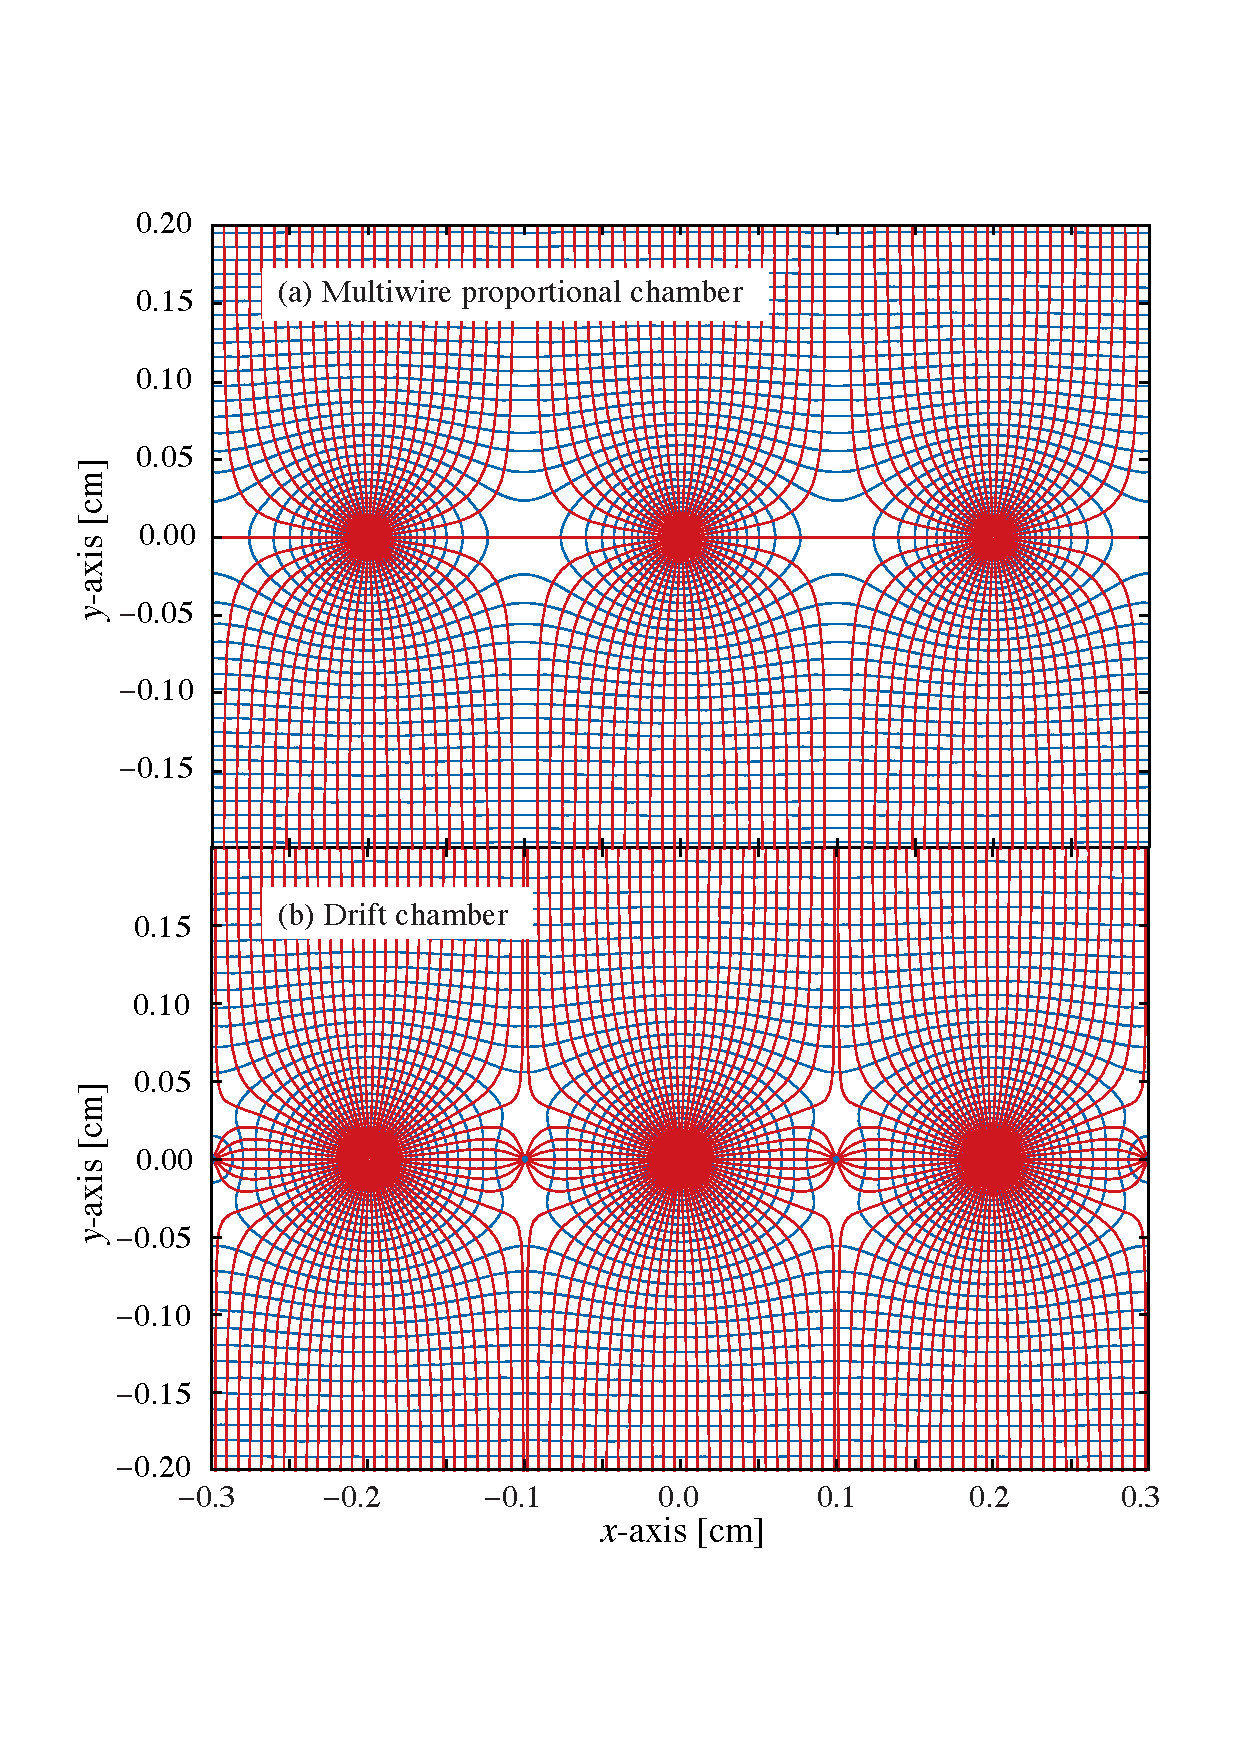
\includegraphics[width=110mm]{Chapter1/figures/mwpcLines.pdf}
	\caption{The difference between MWPC and Drift Chamber field lines. Image from \cite{radiationLengthsBook}.}
	\label{fig:fieldLinesDriftChamber}
\end{center}
\end{figure}

\begin{figure}[htbp]
\begin{center}
	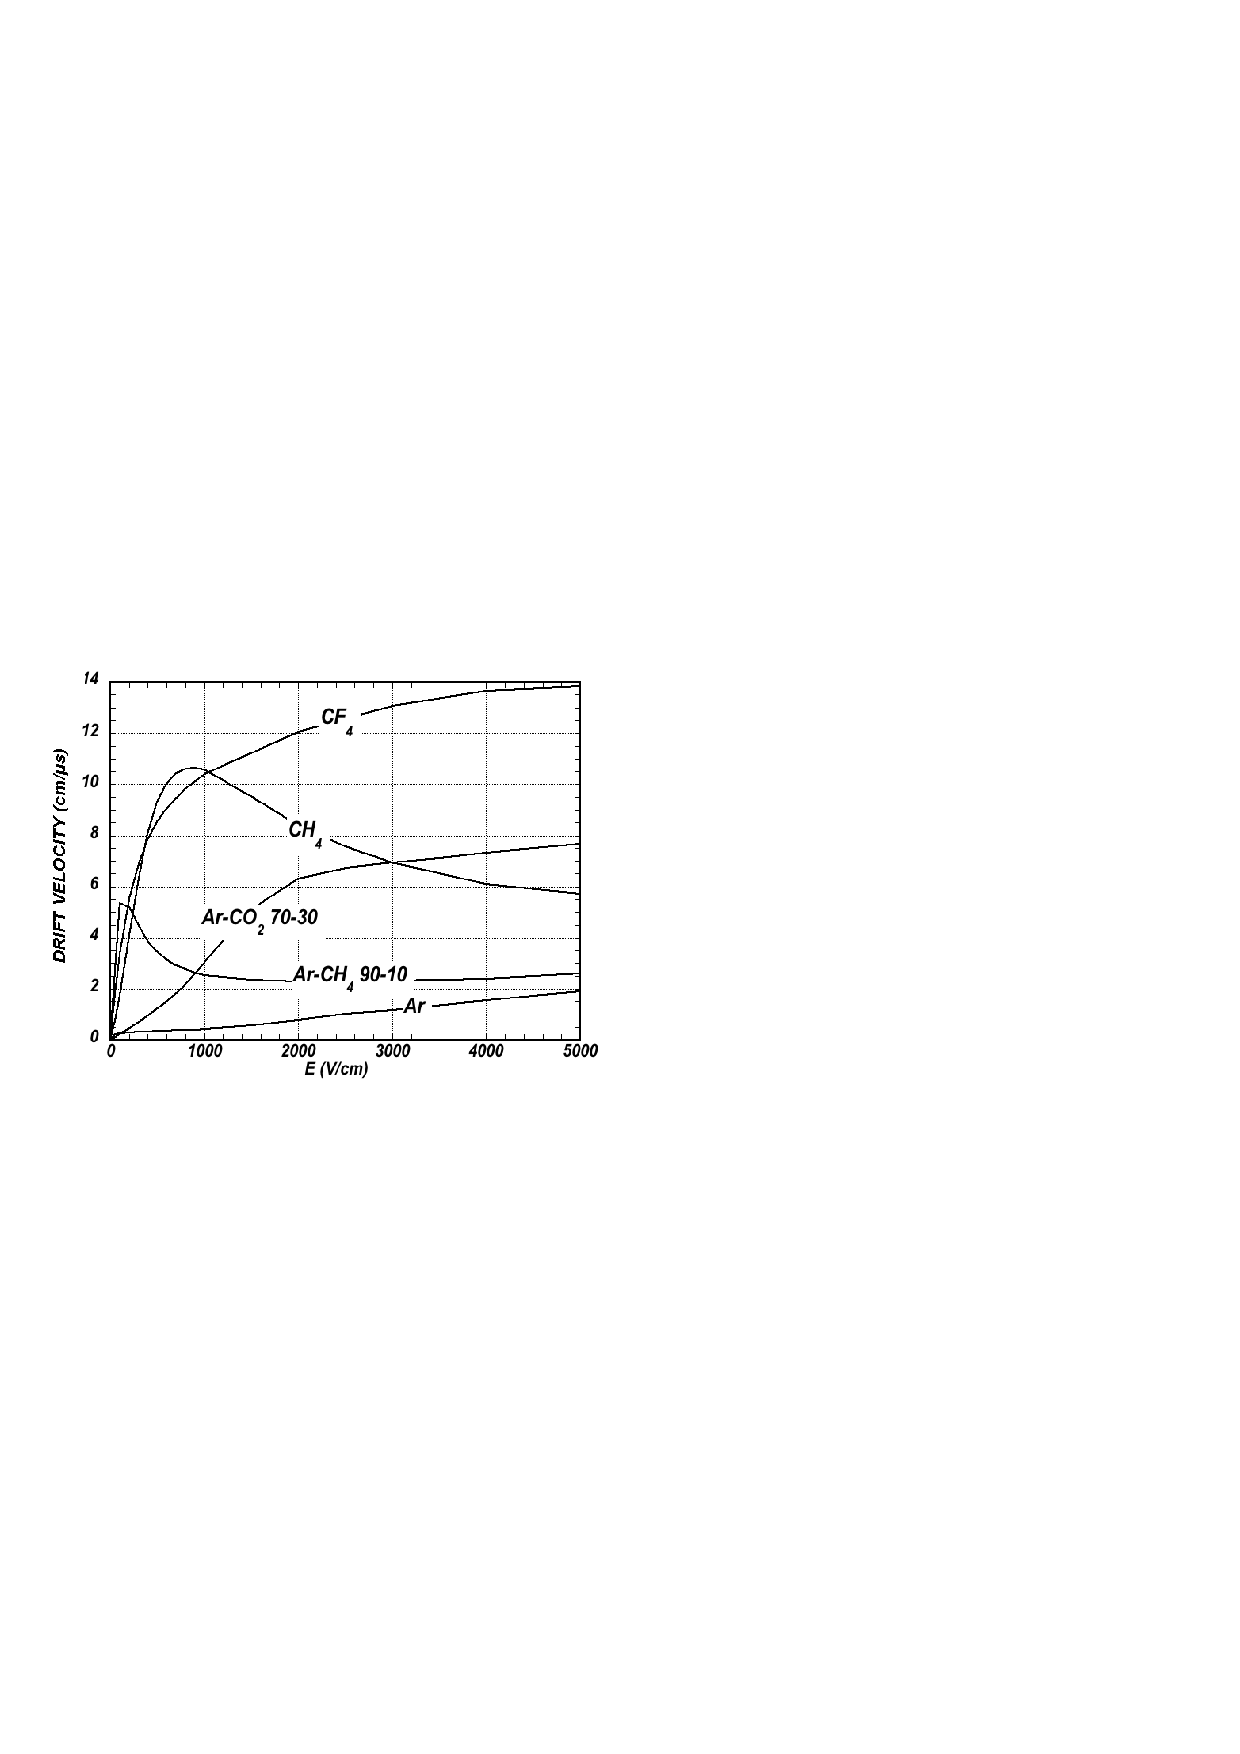
\includegraphics[width=100mm]{Chapter1/figures/driftVelocitiesArgon.pdf}
	\caption{The electron drift velocities for various gases including combinations with Argon. Ar, Ar (90\%) + CH$_{4}$(10\%), Ar (70\%) + CO$_{2}$(30\%), CH$_{4}$ and CF$_{4}$ are shown. Image from \cite{gasDetectors}.}
	\label{fig:driftVelocitiesArgon}
\end{center}
\end{figure}

The TPC is considered the improved drift chamber with the concept introduced in 1976 \cite{gasDetectors}. They employ both concepts of the MWPC and Drift Chambers, using MWPCs to readout charge after being drifted. As a result TPCs can provide a 3-dimensional view of charged particles traversing the detector. Using a uniform electric field applied across the volume ionisation can be drifted, produced from a passing track, to a readout end plate. This provides a 2-dimensional view of the track with the third determined from the drift time. Knowledge of the electron drift velocity, the diffusion in the medium and accurate modelling of the electric field must be well understood in order to provide an accurate description of the track. 

Argon is commonly implemented for TPCs, and with drift speeds of the order of cm/$\mu$s for LAr, good resolutions can be achieved in the drift direction $\sigma(z)$ $\sim$100 $\mu$m. However with large drifting volumes of 1 m and above, high voltages are required. Also coupled with slow drift times $\sim$100 $\mu$s and slow readout, pileup can become an issue with this detector technology. Hence they are not well suited as detectors where high event rates are possible.

It is best to operate these detectors in proportional mode, so that the number of electrons produced remains proportional to the measured signal. However during amplification, avalanches occur that cause further ionisation and further photon emission, introducing additional charge that can result in the loss in proportionality. The removal of these photons is done by the additional of quench gases (such as isobutane, methane or CO$_{2}$) to the noble gas. The high Ultra Violet (UV) photon cross sections of these molecules results in the absorption of the scintillation light and helps maintain proportionality. Another benefit of the addition of the quench gases is the increase in electron drift velocity due to the reduction of the electrons energy and its scattering cross section. The use of quench gases restricts the detection method to ionisation but the implementation of noble gases as scintillation detectors can be employed when high purities are obtained. The effect on the drift velocity in Argon can be seen in figure \ref{fig:driftVelocitiesArgon} \cite{gasDetectors}.

\section{Noble Gases as Scintillation Detectors}
The notion to use noble gases as scintillation materials first arose in 1951 when Gr\"{u}n and Schopper implemented the first noble gas scintillation counter\cite{grunSchopper}. Since then the technology has developed to facilitate the use for nuclear radiation spectrometers, high energy calorimeters and other implementations. The attractiveness of their use as scintillation media is due to several reasons:
\begin{itemize}
	\item High light yields
	\item Transparency to own scintillation light
	\item Fast scintillation light decay times
	\item Good linearity of scintillation yield over $E$ and $dE/dx$
	\item Attainable high purities
	\item Scalability in detectors
\end{itemize}
When a particle deposits energy in the detector medium it transfers its energy to the atoms within the noble gas and will either excite or ionise them. Upon excitation an electron is raised to higher potential, they then can de excite or in denser materials collide with neighbouring atoms and combine to form an excited diatomic molecular state. This excited molecule then subsequently de excites emitting a Ultra Violet (UV) photon, via the process
\begin{equation}
	A^{*} + A \rightarrow A^{*}_{2}
\end{equation} 
\vspace{-5mm}
\begin{equation}
	A^{*}_{2} \rightarrow 2A + h\nu
\end{equation} 
where $A$ represents the noble gas atom, and $A^{*}$ represents the excited state.
The excited diatomic state, $A^{*}_{2}$, can also be formed via ionisation. Upon ionisation a free electron and charged ion pair are created. Again neighbouring atoms can combine to form an ionised molecule, which in turn follows a recombination process with a free electron, via the process
\begin{equation}
	A^{+} + A \rightarrow A^{+}_{2}
\end{equation} 
\vspace{-5mm}
\begin{equation}
	A^{+}_{2} + e^{-} \rightarrow A^{*}_{2}
\end{equation} 
Here $A^{+}$ and $e^{-}$ represent an ionisation state and electron respectively. Upon recombination, an excited molecule remains which de excites again producing a UV photon. The two processes produce a fast and slow scintillation component with relaxation times of the order of 6 ns and 1-1.6 $\mu$s respectively in liquid argon \cite{modesInternal}. This process leading to the photon emission is shown in figure \ref{fig:scintLightDiagram}. The fast and slow components of the scintillation light can allow for Pulse Shape Discrimination (PSD) analysis, which can provide information on incident particles and help discriminate between them in the detector.

\begin{figure}[htbp]
\begin{center}
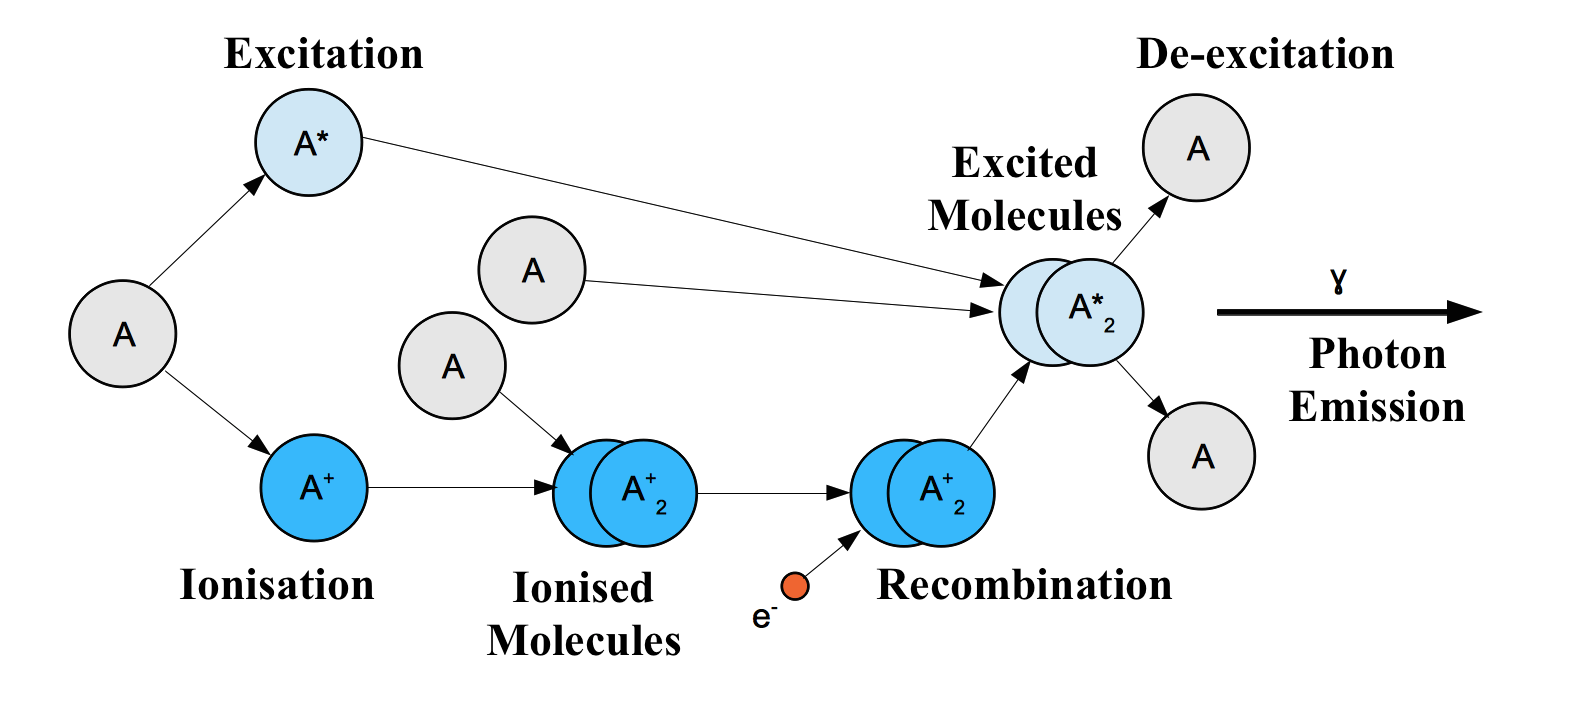
\includegraphics[width=150mm]{Chapter1/figures/scintillationLight2.png}
\caption{A graphical representation of the excitation and ionisation processes in noble gases to produce scintillation light. Image based on figure from \cite{modesInternal}.}
\label{fig:scintLightDiagram}
\end{center}
\end{figure}

High light yields have been achieved for noble gases with scintillation yields of $\sim$46,000 $\gamma$/MeV for gas xenon and $\sim$40,000 $\gamma$/MeV for gas argon \cite{modesInternal}. Coupled with the ability to have very pure gases allows for transport of the scintillation light with the medium. However with wavelengths below 180 nm, it is difficult to detect these photons with current Photo Multiplier Tubes (PMT's) and most detectors employing noble gases use wavelength shifters to absorb and emit the light to a lower frequency, with wavelengths of around 400 nm.

Xenon is considered the most favourable option of the noble gases for scintillator detectors, mainly due to its high atomic number, high density and it containing no radioactive isotopes. Being the most expensive to produce, as the least abundant of the 5, it is therefore best suited for small scale detectors. Argon is a more suitable candidate for larger detector volumes as it is far cheaper and also has good scintillation properties. Contrary to this low atomic numbers can also be favourable for detectors that rely on elastic scattering, such as neutron detection. In this case helium is the superior choice of the noble gases due to its low atomic mass number. As from equation \ref{eq:neutronScatter}, it can be seen that up to 64\% of its kinetic energy can be transferred per scatter for $^{4}$He. Table \ref{tab:elasticScatterNobleGases} shows the energy transfer ratios for various noble gas isotopes, calculated from equation \ref{eq:neutronScatter}.
\begin{table}[htbp]
\begin{center}
  \begin{tabular}{l*{2}{c}r}
  \hline
  \textbf{Noble Gas} & \textbf{Maximum energy transfer} \\
  & \textbf{per scatter}\\
  \hline
  $^{4}$He & 64.0\%\\
  $^{20}$Ne & 18.1\%\\
  $^{40}$Ar & 9.5\%\\
  $^{84}$Kr & 4.7\%\\
  $^{129}$Xe & 3.1\%\\
  \hline
  \end{tabular}
      \caption{The maximum kinetic energy transfer kinematically permitted for various noble gas isotopes. Values based on calculations from equation \ref{eq:neutronScatter}.}
    \label{tab:elasticScatterNobleGases}
\end{center}
    \end{table}
    


